\documentclass[10pt, a4paper]{report}
% !TeX program = xelatex
%==================PREAMBOLO=======================%
%%%%%%%%%%%%%%%%%%%%%%%%%%%%%%%%%%%%%%%%%%%%%%%%%%%%%%%%%%%%%%%%%%%%%%%%%%%%%
%% PREAMBLE
%% Reorganized for readability: packages, colors, custom commands, code
%% listing styles, tcolorbox theorem-like environments and title formatting
%% are grouped by purpose. No functional change was made to the original
%% document: only the order of declarations and the comments were edited.
%%%%%%%%%%%%%%%%%%%%%%%%%%%%%%%%%%%%%%%%%%%%%%%%%%%%%%%%%%%%%%%%%%%%%%%%%%%%%


%%%%%%%%%%%%%%%%%%%%%%%%%%%%%%%%%%%%%%%%%%%%%%%%%%%%%%%%%%%%%%%%%%%%%%%%%%%%%
%% 1. PACKAGES
%%%%%%%%%%%%%%%%%%%%%%%%%%%%%%%%%%%%%%%%%%%%%%%%%%%%%%%%%%%%%%%%%%%%%%%%%%%%%

% --- Encoding, language and fonts ---------------------------------------
\usepackage[utf8]{inputenc}
\usepackage[T1]{fontenc}
\usepackage[english]{babel}
\usepackage{mathpazo}          % Palatino font, replaces lmodern to match the image's serif style
\usepackage[scaled]{helvet}    % Helvetica, used for section/subsection titles

% --- Page layout and headers/footers ------------------------------------
\usepackage[paper=a4paper,left=25mm,right=25mm,bottom=25mm,top=25mm]{geometry}
\usepackage{fancyhdr}
\usepackage[Rejne]{fncychap}
\usepackage{titlesec}
\usepackage{titletoc}
\usepackage{needspace}

% --- Math ----------------------------------------------------------------
\usepackage{amsmath}
\usepackage{amssymb}
\usepackage{amsfonts}
\usepackage{mathtools}
\usepackage{mathrsfs}
\usepackage{stmaryrd}
\usepackage{nicefrac, xfrac}

% --- Graphics and TikZ -----------------------------------------------------
\usepackage{graphicx}          % Required for inserting images
\usepackage[export]{adjustbox}
\usepackage{pdfpages}
\usepackage{tikz}
\usepackage{tikz-3dplot}
\usepackage{tikz-cd}
\usepackage{pgfplots}
\usepackage{pgf-pie}
\usetikzlibrary{positioning}

% --- Colors and colored boxes ---------------------------------------------
\usepackage[table,xcdraw]{xcolor}
\usepackage[most]{tcolorbox}
\tcbuselibrary{theorems}

% --- Lists, layout helpers and decorations --------------------------------
\usepackage[shortlabels]{enumitem}
\usepackage{wrapfig}
\usepackage{multicol}
\usepackage{moresize}
\usepackage{fourier-orns}       % Decorative ornaments (used by \flowerLine, \eqImportante)
\usepackage{psvectorian}        % Decorative vectorial ornaments
\usepackage{lipsum}             % Placeholder ("dummy") text
\usepackage{blindtext}          % Placeholder ("dummy") text

% --- Code listings ---------------------------------------------------------
\usepackage{listings}
\usepackage{minted}

% --- Miscellaneous ---------------------------------------------------------
\usepackage{hyperref}


%%%%%%%%%%%%%%%%%%%%%%%%%%%%%%%%%%%%%%%%%%%%%%%%%%%%%%%%%%%%%%%%%%%%%%%%%%%%%
%% 2. COLOR DEFINITIONS
%%%%%%%%%%%%%%%%%%%%%%%%%%%%%%%%%%%%%%%%%%%%%%%%%%%%%%%%%%%%%%%%%%%%%%%%%%%%%

% --- General purpose colors ---
\definecolor{light-gray}{gray}{0.95}
\definecolor{darkgreen}{HTML}{008000}
\definecolor{g}{RGB}{60, 50, 50}

% --- "Sapienza" theme colors ---
\definecolor{sapienza}{HTML}{660f1d}
\definecolor{lightSapienza}{HTML}{e3d3d5}

% --- Cover / decorative colors ---
\definecolor{cop}{HTML}{f7ecd7}
\definecolor{copAut}{HTML}{ababab}
\definecolor{copAut2}{HTML}{c3c3e6}
\definecolor{purcop}{HTML}{d0d3db}
\definecolor{cartaRiciclata}{HTML}{fcfcf7}

% --- Colors used for C / C++ code listings ---
\definecolor{mGreen}{rgb}{0,0.6,0}
\definecolor{mGray}{rgb}{0.5,0.5,0.5}
\definecolor{mPurple}{rgb}{0.58,0,0.82}
\definecolor{backgroundColour}{rgb}{0.95,0.95,0.92}


%%%%%%%%%%%%%%%%%%%%%%%%%%%%%%%%%%%%%%%%%%%%%%%%%%%%%%%%%%%%%%%%%%%%%%%%%%%%%
%% 3. CUSTOM COMMANDS
%%%%%%%%%%%%%%%%%%%%%%%%%%%%%%%%%%%%%%%%%%%%%%%%%%%%%%%%%%%%%%%%%%%%%%%%%%%%%

% --- Colored text shortcuts ------------------------------------------------
\newcommand{\redText}[1]{\color{red}#1\color{black}}
\newcommand{\blueText}[1]{\color{blue}#1\color{black}}
\newcommand{\greenText}[1]{\color{darkgreen}#1\color{black}}
\newcommand{\sapText}[1]{\color{sapienza}#1\color{black}}
\newcommand{\textg}[1]{\color{g}{\textbf{#1}}\color{black}}

% --- Inline code / shell snippets -------------------------------------------
\newcommand{\code}[1]{\colorbox{light-gray}{\texttt{#1}}}
\newcommand{\codee}[1]{\colorbox{white}{\texttt{#1}}}
\newcommand{\shell}[1]{\colorbox{black}{\textcolor{white}{\texttt{#1}}}}
\newcommand{\boxedMath}[1]{\begin{tabular}{|c|}\hline \texttt{#1} \\ \hline\end{tabular} :}

% --- Highlighted paragraph boxes --------------------------------------------
\newcommand\greybox[1]{%
  \vskip\baselineskip%
  \par\noindent\colorbox{light-gray}{%
    \begin{minipage}{\textwidth}#1\end{minipage}%
  }%
  \vskip\baselineskip%
}
\newcommand\sapbox[1]{%
  \vskip\baselineskip%
  \par\noindent\colorbox{lightSapienza}{%
    \begin{minipage}{\textwidth}#1\end{minipage}%
  }%
  \vskip\baselineskip%
}

% --- Statement labels (theorem/definition/etc. headers as plain text) ------
\newcommand{\teo}[1]{{\large\color{sapienza}\textbf{Teorema #1 :\hphantom{a}}}}
\newcommand{\defi}[1]{{\large\color{sapienza}\textbf{Definizione #1 :\hphantom{a}}}}
\newcommand{\prop}[1]{{\color{sapienza}\textbf{Proposizione #1 :\hphantom{a}}}}
\newcommand{\lemma}[1]{{\color{sapienza}\textbf{Lemma #1 :\hphantom{a}}}}
\newcommand{\claim}[1]{{\color{sapienza}\textbf{Claim #1 :\hphantom{a}}}}
\newcommand{\dimo}[1]{{\color{sapienza}\textbf{Dimostrazione #1 :\hphantom{a}}}}
\newcommand{\acc}{\\\hphantom{}\\}
\newcommand{\esempio}[1]{{\acc\large\color{sapienza}\textbf{Esempio #1 \hphantom{a}}\acc}}

% --- Number sets and blackboard-bold symbols --------------------------------
\newcommand{\N}{{\mathbb N}}
\newcommand{\Z}{{\mathbb Z}}
\newcommand{\R}{{\mathbb R}}
\newcommand{\C}{{\mathbb C}}
\newcommand{\K}{{\mathbb K}}
\newcommand{\quat}{{\mathbb H}}
\newcommand{\Prob}{{\mathbb P}}
\newcommand{\VA}{{\mathbb E}}

% --- Calligraphic / script symbols ------------------------------------------
\newcommand{\Sn}{{\mathcal S_n}}
\newcommand{\An}{{\mathcal A_n}}
\newcommand{\E}{{\mathcal E}}
\newcommand{\B}{{\mathcal B}}

% --- Bold vector/greek symbols ----------------------------------------------
\newcommand{\btheta}{{\boldsymbol{\theta}}}
\newcommand{\btau}{{\boldsymbol{\tau}}}
\newcommand{\bomega}{{\boldsymbol{\omega}}}
\newcommand{\Bomega}{{\boldsymbol{\Omega}}}
\newcommand{\bmu}{{\boldsymbol{\mu}}}
\newcommand{\brho}{{\boldsymbol{\rho}}}
\newcommand{\bnu}{{\boldsymbol{\nu}}}
\newcommand{\bsigma}{{\boldsymbol{\sigma}}}
\newcommand{\blambda}{{\boldsymbol{\lambda}}}

% --- Dotted mechanics symbols (velocity/acceleration notation) -------------
\newcommand{\dq}{{\dot{\mathbf q}}}
\newcommand{\de}{{\dot{\mathbf e}}}
\newcommand{\dy}{{\dot{\mathbf y}}}
\newcommand{\ddq}{{\ddot{\mathbf q}}}
\newcommand{\ddy}{{\ddot{\mathbf y}}}
\newcommand{\ve}{{\bar v}}

% --- Group theory / algebra operators ---------------------------------------
\newcommand{\aut}{{\text{Aut}}}
\newcommand{\Span}{{\text{Span}}}
\newcommand{\End}{{\text{End}}}
\newcommand{\cen}{{\text{Centro}}}
\newcommand{\norm}{{\unlhd}}
\newcommand{\ciclS}{{\left \langle }}
\newcommand{\ciclE}{{\right \rangle }}
\newcommand{\bra}[1]{\langle #1 \rangle}
\newcommand{\mcm}{{\text{mcm}}}
\newcommand{\MCD}{{\text{MCD}}}
\newcommand{\rg}{{\text{rg}}}
\newcommand{\supp}{{\text{Supp}}}

% --- Complexity theory symbols -----------------------------------------------
\newcommand{\ridFunc}{{f:\Sigma^*\rightarrow \Sigma^*}}
\newcommand{\rid}{{\le_m^P}}
\newcommand{\blank}{{\sqcup}}

% --- Miscellaneous math symbols and utilities -------------------------------
\newcommand{\quadBrack}[1]{ \llbracket #1 \rrbracket }
\newcommand{\notimplies}{%
  \mathrel{{\ooalign{\hidewidth$\not\phantom{=}$\hidewidth\cr$\implies$}}}}
\newcommand{\tc}{{\text{ tale che }}}
\newcommand{\spaz}{{\text{\hphantom{aa}}}}

% --- Decorative separators ---------------------------------------------------
\newcommand{\flowerLine}{ \begin{center}\decofourleft\hphantom{ }\decoone\hphantom{ }\decofourright\hphantom{}\hphantom{aa}
\decofourleft\hphantom{ }\decoone\hphantom{ }\decofourright\hphantom{}\hphantom{aa}
\decofourleft\hphantom{ }\decoone\hphantom{ }\decofourright\hphantom{}\hphantom{aa}
\decofourleft\hphantom{ }\decoone\hphantom{ }\decofourright\hphantom{}\hphantom{aa} 
\decofourleft\hphantom{ }\decoone\hphantom{ }\decofourright\hphantom{}\hphantom{aa}
\decofourleft\hphantom{ }\decoone\hphantom{ }\decofourright\hphantom{}\hphantom{aa}
\decofourleft\hphantom{ }\decoone\hphantom{ }\decofourright\hphantom{}\hphantom{aa}
\decofourleft\hphantom{ }\decoone\hphantom{ }\decofourright\hphantom{}\hphantom{aa}
\decofourleft\hphantom{ }\decoone\hphantom{ }\decofourright\hphantom{}\hphantom{aa}
\end{center}}
\newcommand{\eqImportante}[1]{\begin{center}\huge\lefthand\hphantom{a}
    \normalsize\texttt{#1}
    \hphantom{aaa}\huge\righthand\end{center}}


%%%%%%%%%%%%%%%%%%%%%%%%%%%%%%%%%%%%%%%%%%%%%%%%%%%%%%%%%%%%%%%%%%%%%%%%%%%%%
%% 4. PAGE STYLE (HEADER / FOOTER)
%%%%%%%%%%%%%%%%%%%%%%%%%%%%%%%%%%%%%%%%%%%%%%%%%%%%%%%%%%%%%%%%%%%%%%%%%%%%%
\fancyhf{}
\pagestyle{fancy}
\renewcommand{\headrulewidth}{0.4pt}


%%%%%%%%%%%%%%%%%%%%%%%%%%%%%%%%%%%%%%%%%%%%%%%%%%%%%%%%%%%%%%%%%%%%%%%%%%%%%
%% 5. CODE LISTING STYLES (C / C++)
%%%%%%%%%%%%%%%%%%%%%%%%%%%%%%%%%%%%%%%%%%%%%%%%%%%%%%%%%%%%%%%%%%%%%%%%%%%%%
% The following styles configure the `listings` package for displaying
% C and C++ source code with syntax highlighting.

\lstdefinestyle{CStyle}{
    backgroundcolor=\color{backgroundColour},   
    commentstyle=\color{mGreen},
    keywordstyle=\color{magenta},
    numberstyle=\tiny\color{mGray},
    stringstyle=\color{mPurple},
    basicstyle=\footnotesize,
    breakatwhitespace=false,         
    breaklines=true,                 
    captionpos=b,                    
    keepspaces=true,                 
    numbers=left,                    
    numbersep=5pt,                  
    showspaces=false,                
    showstringspaces=false,
    showtabs=false,                  
    tabsize=2,
    language=C
}

\lstdefinestyle{CppStyle}{
    backgroundcolor=\color{backgroundColour},   
    commentstyle=\color{mGreen}\ttfamily,
    morecomment=[l][\color{magenta}]{\#}
    keywordstyle=\color{blue}\ttfamily,
    numberstyle=\tiny\color{mGray},
    stringstyle=\color{red}\ttfamily,
    basicstyle=\ttfamily,
    breakatwhitespace=false,         
    breaklines=true,                 
    captionpos=b,                    
    keepspaces=true,                 
    numbers=left,                    
    numbersep=5pt,                  
    showspaces=false,                
    showstringspaces=false,
    showtabs=false,                  
    tabsize=2,
    language=C
}

% Global default `listings` configuration (applied when no style is selected)
\lstset{language=C++,
                basicstyle=\ttfamily,
                keywordstyle=\color{blue}\ttfamily,
                stringstyle=\color{red}\ttfamily,
                commentstyle=\color{green}\ttfamily,
                morecomment=[l][\color{magenta}]{\#}
}


%%%%%%%%%%%%%%%%%%%%%%%%%%%%%%%%%%%%%%%%%%%%%%%%%%%%%%%%%%%%%%%%%%%%%%%%%%%%%
%% 6. TCOLORBOX THEOREM-LIKE ENVIRONMENTS
%%%%%%%%%%%%%%%%%%%%%%%%%%%%%%%%%%%%%%%%%%%%%%%%%%%%%%%%%%%%%%%%%%%%%%%%%%%%%
% Each environment below renders a boxed, numbered statement (definition,
% theorem, proposition, ...) with a "tab" style title in the top-left
% corner, following the same visual template.

\newtcbtheorem[number within=section]{boxdefinition}{Definition}{
    enhanced,
    before skip=15pt, after skip=15pt,
    colback=white,                          % white background for the text
    colframe=sapienza!50!black!30,          % border color (light green/gray)
    fonttitle=\bfseries,
    coltitle=black,
    % Style of the top-left "tab"
    attach boxed title to top left={xshift=10mm, yshift=-3.5mm, yshifttext=-1mm},
    boxed title style={
        colframe=sapienza!50!black!30,
        arc=3mm,
        outer arc=3mm,
        left=10pt, right=10pt,
        top=2pt, bottom=2pt,
        % Green gradient shading, as in the reference image
        interior style={left color=sapienza!20, right color=sapienza!40}
    },
    % Rounding of the main box
    arc=4mm,
    separator sign none,                    % removes the automatic colon so it can be added manually in the title
    description font=\normalfont\bfseries,
    description delimiters={: }{ }          % formats the title as "Definition 2.1: Title"
}{def}

\newtcbtheorem[number within=section]{boxtheorem}{Theorem}{
    enhanced,
    before skip=15pt, after skip=15pt,
    colback=white,
    colframe=sapienza!50!black!30,
    fonttitle=\bfseries,
    coltitle=black,
    attach boxed title to top left={xshift=10mm, yshift=-3.5mm, yshifttext=-1mm},
    boxed title style={
        colframe=sapienza!50!black!30,
        arc=3mm,
        outer arc=3mm,
        left=10pt, right=10pt,
        top=2pt, bottom=2pt,
        interior style={left color=sapienza!20, right color=sapienza!40}
    },
    arc=4mm,
    separator sign none,
    description font=\normalfont\bfseries,
    description delimiters={: }{ }
}{def}

\newtcbtheorem[number within=section]{boxproposition}{Proposition}{
    enhanced,
    before skip=15pt, after skip=15pt,
    colback=white,
    colframe=sapienza!50!black!30,
    fonttitle=\bfseries,
    coltitle=black,
    attach boxed title to top left={xshift=10mm, yshift=-3.5mm, yshifttext=-1mm},
    boxed title style={
        colframe=sapienza!50!black!30,
        arc=3mm,
        outer arc=3mm,
        left=10pt, right=10pt,
        top=2pt, bottom=2pt,
        interior style={left color=sapienza!30, right color=sapienza!50}
    },
    arc=4mm,
    separator sign none,
    description font=\normalfont\bfseries,
    description delimiters={: }{ }
}{def}

\newtcbtheorem[number within=section]{boxequation}{Equation}{
    enhanced,
    before skip=15pt, after skip=15pt,
    colback=white,
    colframe=sapienza!50!black!30,
    fonttitle=\bfseries,
    coltitle=black,
    attach boxed title to top left={xshift=10mm, yshift=-3.5mm, yshifttext=-1mm},
    boxed title style={
        colframe=sapienza!50!black!30,
        arc=3mm,
        outer arc=3mm,
        left=10pt, right=10pt,
        top=2pt, bottom=2pt,
        interior style={left color=sapienza!30, right color=sapienza!50}
    },
    arc=4mm,
    separator sign none,
    description font=\normalfont\bfseries,
    description delimiters={: }{ }
}{def}

\newtcbtheorem[number within=section]{boxlemma}{Lemma}{
    enhanced,
    before skip=15pt, after skip=15pt,
    colback=white,
    colframe=sapienza!50!black!30,
    fonttitle=\bfseries,
    coltitle=black,
    attach boxed title to top left={xshift=10mm, yshift=-3.5mm, yshifttext=-1mm},
    boxed title style={
        colframe=sapienza!50!black!30,
        arc=3mm,
        outer arc=3mm,
        left=10pt, right=10pt,
        top=2pt, bottom=2pt,
        interior style={left color=sapienza!30, right color=sapienza!50}
    },
    arc=4mm,
    separator sign none,
    description font=\normalfont\bfseries,
    description delimiters={: }{ }
}{def}

\newtcbtheorem[number within=section]{boxobservation}{Observation}{
    enhanced,
    before skip=15pt, after skip=15pt,
    colback=white,
    colframe=sapienza!50!black!30,
    fonttitle=\bfseries,
    coltitle=black,
    attach boxed title to top left={xshift=10mm, yshift=-3.5mm, yshifttext=-1mm},
    boxed title style={
        colframe=sapienza!50!black!30,
        arc=3mm,
        outer arc=3mm,
        left=10pt, right=10pt,
        top=2pt, bottom=2pt,
        interior style={left color=sapienza!30, right color=sapienza!50}
    },
    arc=4mm,
    separator sign none,
    description font=\normalfont\bfseries,
    description delimiters={: }{ }
}{def}

\newtcbtheorem[number within=section]{boxpostulate}{Postulate}{
    enhanced,
    before skip=15pt, after skip=15pt,
    colback=white,
    colframe=sapienza!50!black!30,
    fonttitle=\bfseries,
    coltitle=black,
    attach boxed title to top left={xshift=10mm, yshift=-3.5mm, yshifttext=-1mm},
    boxed title style={
        colframe=sapienza!50!black!30,
        arc=3mm,
        outer arc=3mm,
        left=10pt, right=10pt,
        top=2pt, bottom=2pt,
        interior style={left color=sapienza!30, right color=sapienza!50}
    },
    arc=4mm,
    separator sign none,
    description font=\normalfont\bfseries,
    description delimiters={: }{ }
}{def}


%%%%%%%%%%%%%%%%%%%%%%%%%%%%%%%%%%%%%%%%%%%%%%%%%%%%%%%%%%%%%%%%%%%%%%%%%%%%%
%% 7. SECTION / SUBSECTION TITLE FORMATTING
%%%%%%%%%%%%%%%%%%%%%%%%%%%%%%%%%%%%%%%%%%%%%%%%%%%%%%%%%%%%%%%%%%%%%%%%%%%%%

% Section titles: Helvetica, large bold number, colored rule underneath
\titleformat{\section}
  {\needspace{3\baselineskip} % requires at least 3 lines of free space before the title
   \fontfamily{phv}\selectfont\huge\bfseries} 
  {\color{sapienza}\fontsize{20}{20}\selectfont\thesection} 
  {12pt} 
  {} 
  [\vspace{2pt}\nopagebreak\color{sapienza!40}\hrule height 3pt]

% Subsection titles: same style, slightly smaller
\titleformat{\subsection}
  {\needspace{2\baselineskip} % requires at least 2 lines of free space before the title
   \fontfamily{phv}\selectfont\Large\bfseries} 
  {\color{sapienza}\fontsize{16}{16}\selectfont\thesubsection} 
  {12pt} 
  {} 
  [\vspace{2pt}\nopagebreak\color{sapienza!40}\hrule height 1.5pt]
\newcommand{\y}{{\mathbf y}}
\newcommand{\q}{{\mathbf q}}
\usepackage{algorithm}
\usepackage{algpseudocode}
 \usepackage{multirow}
\newcommand{\titolo}{Elective in Robotics}

 %TOGLI COMMENTO SE USI XELATEX
%\usepackage{fontspec}
\title{\titolo} %========TITOLO========%
\author{Marco Casu}
\date{\vspace{-5ex}}
\begin{document}

%==================COPERTINA=======================%
\begin{titlepage}
    \centering
     
    
\includegraphics[width=0.6\textwidth]{../../preamble/Stemma_sapienza.png} 
    \par\vspace{2.5cm}
    
    {\huge \textsc{``Sapienza'' University of Rome}}
    \par\vspace{0.5cm}
    {\Large \textsc{Faculty of Information Engineering,\\ Computer Science and Statistics}} \\[1.5ex]
    {\Large \textsc{Department of Computer, Control\\ and Management Engineering}}
    \\[1.5ex]
    {\Large \textsc{Master's degree in Artificial Intelligence and Robotics
}}
    
    \vspace{2.5cm} % Spazio verticale regolabile
    
    \rule{\textwidth}{2pt} \\
    \vspace{0.5cm}
    {\fontsize{35}{70} \selectfont \textbf{\titolo}} \\
    \vspace{0.35cm}
    \rule{\textwidth}{2pt}
    
    \vspace{0.5cm}
    {\Large Lecture notes}
    
    \vfill % Spinge il contenuto successivo in basso
    
    {\textit{Author}} \\
    {\large{Marco Casu}}
    
    \vspace{2cm}
    
    {\large \today}
    
\end{titlepage}
%===================FINE COPERTINA======================%
\newpage
%\pagecolor{cartaRiciclata}%\setmainfont{Algerian}
\Large
This document summarizes and presents the topics for the \titolo course for the Master's degree in Artificial Intelligence and Robotics at Sapienza University of Rome. The document is free for any use. If the reader notices any typos, they are kindly requested to report them to the author.
\vfill
\begin{figure}[h!]
    \raggedright
    
\includegraphics[width=0.4\textwidth,right ]{../../preamble/tomodachi.pdf} 
\end{figure}
\newpage %\setmainfont{Times New Roman}
\normalsize

\tableofcontents 
\newpage

%==================FOOTER e HEADER=======================%
\fancyhf{}
\fancyhead[L]{\nouppercase{\leftmark}}
\fancyhead[R]{Section \thesection}
\fancyfoot[C]{\thepage}
\fancyfoot[L]{\titolo}
\fancyfoot[R]{ Marco Casu}
%\fancyfoot[R]{\setmainfont{Palace Script MT}\huge Marco Casu \setmainfont{Times New Roman}}
%==================FOOTER e HEADER=======================%
%==================INIZIO======================%
\part{Modeling and Control of Multi-Rotor UAVs}
\chapter{Introduction}
UAVs stands for \textbf{Unmanned Aerial Vehicles}, also known with other names depending on the domain, like \textit{RPVs (Remotely Piloted Vehicles)} in the military domain, or \textit{Drones} in common parlance. We will use all of the three names indistinctively. The methods presented are valid also for remotely operated or autonomous vehicles (at different levels of autonomy).\bigskip

The term UAVs refers to a broad category of vehicles, in general, any aerial vehicle without a pilot on board is a UAV. We will examine UAVs composed of multiple rotors, in particular \textbf{quadrotors}.
\begin{figure}[H]
    \centering
    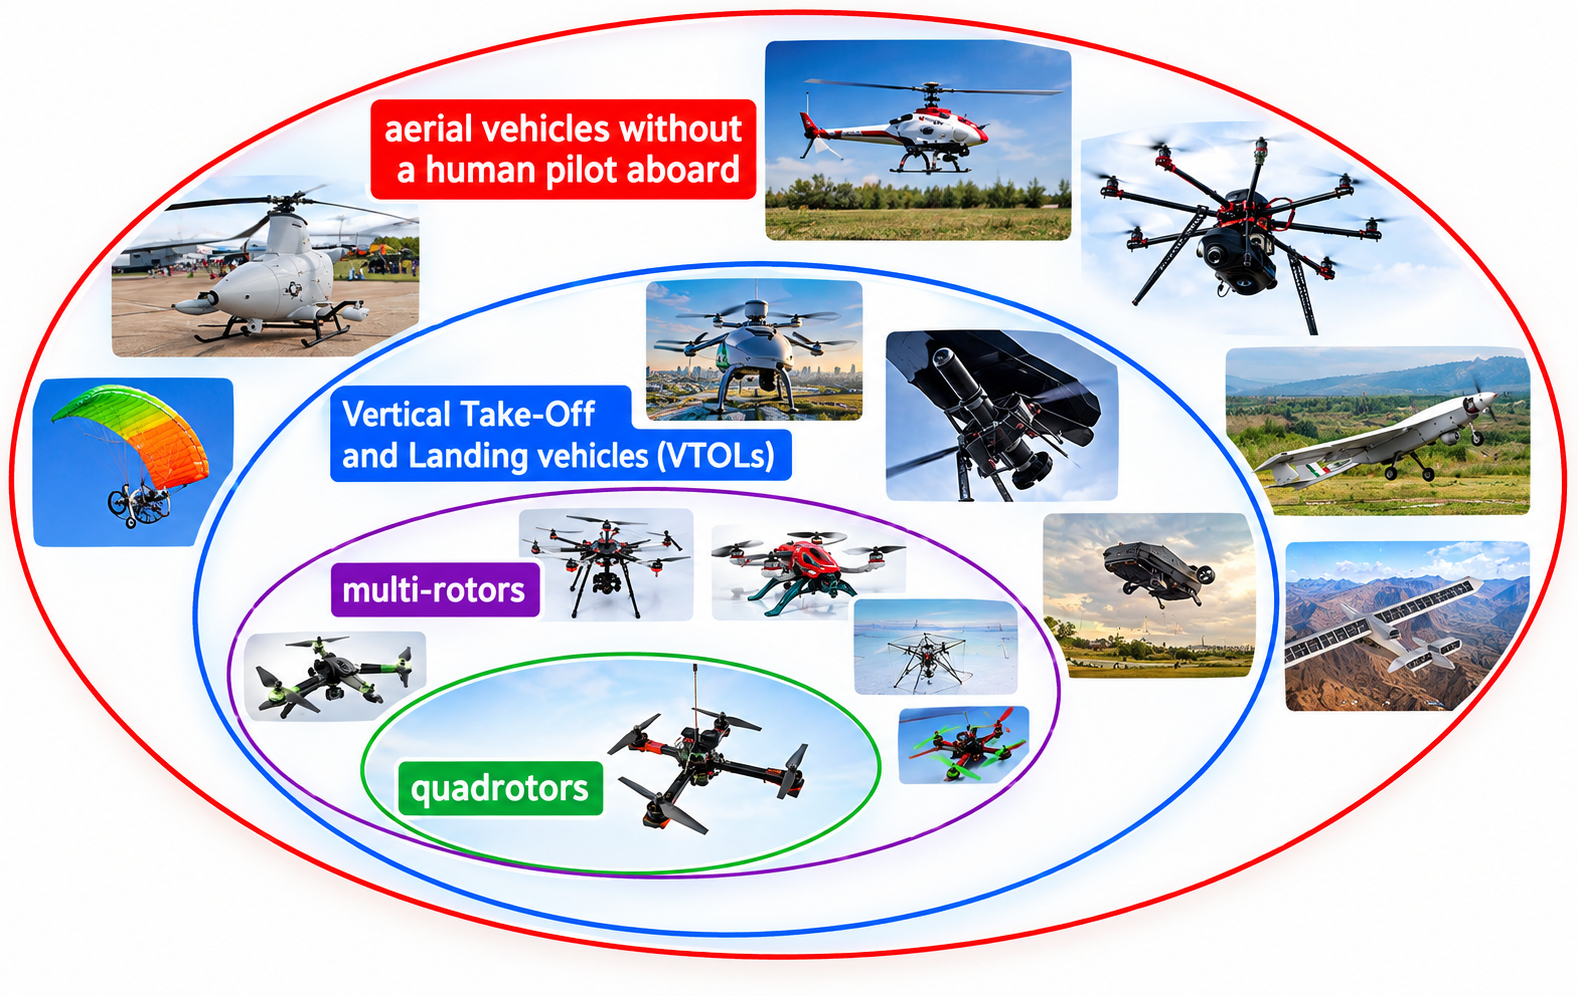
\includegraphics[width=0.7\textwidth ]{images/design based classification.png}
    \caption{Design-based classification.}
\end{figure}
The quadrotors are used in various situations:\begin{itemize}
    \item inspection, maintenance,
    \item communication networks,
    \item search and rescue operations,
    \item aerial transportation, manipulation.
\end{itemize}
These activities require a vertical, stationary and slow flight. A quadrotor is characterized by an high maneuverability, can remain suspended in the air without moving (hovering), and perform a \textit{vertical take-off and landing (VTOL)}, differently from other vehicles like airplanes, that requires an horizontal movement in order to take-off and land.
\section{Modeling}
We call VTOLs the vehicles that can perform a vertical take-off and landing, these are modeled with the North-East-Down (NED) reference frame:
\begin{figure}[H]
    \centering
    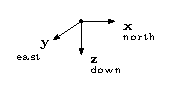
\includegraphics[width=0.3\textwidth ]{images/NEDframe.eps}
    \caption{The NED reference frame.}
    \label{NED}
\end{figure}
\noindent This frame, often called $SR_i$, has the $\mathbf k$ axis pointing down to the center of the Earth. According to the dynamics of rigid bodies given by the Newton-Euler formalism, the translational dynamics of a body in the $SR_i$ frame is given by\begin{equation}\label{sum_forces}
    \sum_j \mathbf F_j = m\dot {\mathbf V}
\end{equation}
where $\mathbf F_j$ are the external forces applied to the center of mass, and $\dot {\mathbf V}$ is the acceleration of the center of mass expressed in $SR_i$. The rotational dynamics is given by\begin{equation}\label{sum_moments}
     \sum_j \mathbf  M_j = J\dot{\boldsymbol{\Omega}} + \boldsymbol{\Omega} \times J \boldsymbol{\Omega}
\end{equation}
where $\mathbf M_j$ are the external moments acting on the center of mass, $\boldsymbol{\Omega}$ is the angular velocity of the body expressed in the body frame, denoted $SR_b$ and $J$ is the inertia tensor, also expressed in $SR_b$.
\begin{figure}[H]
    \centering
    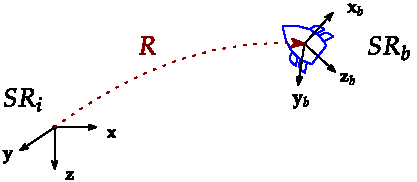
\includegraphics[width=0.7\textwidth ]{images/bodyframe.pdf}
    \caption{$SR_b$ is the reference frame attached to the center of mass of the vehicle, $R$ is the rotation matrix between the two frames.}
    \label{NED}
\end{figure}
\noindent A more explicit expression of the forces in Equation \eqref{sum_forces} is the following:\begin{equation}
    m\dot {\mathbf V} =  -T R\mathbf k
    +\mathbf F_e(\mathbf V,\dot{\mathbf V},\boldsymbol{\Omega},\dot{\boldsymbol{\Omega}},\mathbf d(t))
    +R\Sigma_R\btau
\end{equation}
where:\begin{itemize}
    \item $\mathbf d(t)$ are the external disturbances that do not depend on 
    the vehicle's state.
    \item $\mathbf F_e$ are the external forces, that depend on the state.
    \item $T$ is the \textbf{thrust}, that depends on the number and allocation of the rotors, while $\mathbf -k$ is the direction pointing upward (according to the NED frame as in Figure \ref{NED}). $R$ is the rotation matrix that describes the orientation of our vehicle with respect to the fixed NED frame $SR_i$,
    \item hence the product $-T R\mathbf k$ is the main upward thrust.
    \item $\btau$ is the torque generated by the propellers.
    \item $R\Sigma_R\btau$ are the parasitic forces generated by the rotors/actuators. The coupling matrix $\Sigma_R$ maps the torques/rotations of the motors into small translational lateral forces (then rotated into $SR_I$ via $R$).
\end{itemize}
We know that the derivative of the rotation matrix $R$ depends on the skew-symmetric matrix of the angular velocity:\begin{equation}
    \dot R= R S(\boldsymbol{\Omega})
\end{equation}
$S(\boldsymbol{\Omega})$ is important since it appears in the explicit expression of the term $ J\dot{\boldsymbol{\Omega}} $ in Equation \eqref{sum_moments}:
\begin{equation}
    J\dot{\boldsymbol{\Omega}}=-S(\boldsymbol{\Omega})J\boldsymbol{\Omega}+\btau+
    \btau_e(\mathbf V,\dot{\mathbf V},\boldsymbol{\Omega},\dot{\boldsymbol{\Omega}},\mathbf d(t))+ \btau_g+ 
    \Sigma_T T \mathbf k
\end{equation}
where:\begin{itemize}
    \item $\btau_e$ are the torques induced by the external forces.
    \item $\Sigma_T T \mathbf k$ is the parasitic moment due to the application of the thrust $T$ if the thrust line does not pass perfectly through the center of mass (constructive misalignment). $\Sigma_T$ is a matrix that represents the geometric misalignment between the effective axis of the total thrust $T$ and the center of mass of the vehicle. If the thrust vector does not pass exactly through the center of gravity, it generates a parasitic torque proportional to the thrust itself.
    \item $\btau_g$ is the internal gyroscopic moment due to the inertia of the propellers rotating at high speed (particularly relevant in quadcopters when they change attitude rapidly).
\end{itemize}
We denote $\vec{\mathbf T}=-T\mathbf k_b$ the push in the opposite direction of $\mathbf k_b$ expressed in the vehicle frame $SR_b$. 
\begin{figure}[H]
    \centering
    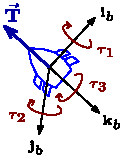
\includegraphics[width=0.2\textwidth ]{images/thrust.pdf}
\end{figure}
\end{document}